\documentclass[lettersize,journal]{IEEEtran}
\usepackage{amsmath,amsfonts}
\usepackage{algorithmic}
\usepackage{array}
\usepackage{subcaption}
\usepackage{textcomp}
\usepackage{stfloats}
\usepackage{url}
\usepackage{verbatim}
\usepackage{booktabs}
\usepackage{multirow}
\usepackage{graphicx}
\usepackage{colortbl}
\usepackage[table,xcdraw]{xcolor}
\usepackage{tikz}
\usepackage{titlesec}
\usepackage{authblk}
\usepackage{marvosym}
\usetikzlibrary{positioning, calc}
\usetikzlibrary{arrows}
\newcolumntype{P}[1]{>{\raggedright\arraybackslash}p{#1}}

\hyphenation{op-tical net-works semi-conduc-tor IEEE-Xplore}
\def\BibTeX{{\rm B\kern-.05em{\sc i\kern-.025em b}\kern-.08em
    T\kern-.1667em\lower.7ex\hbox{E}\kern-.125emX}}
\usepackage{balance}
\begin{document}
\title{bnmetamodel 2.0}



\author[1]{T. Griffiths\thanks{\textsuperscript{\Cross}Corresponding author: t.griffiths20@imperial.ac.uk}}
\author[2]{Z. Xuereb Conti}
\author[1]{M. Bluck}

\affil[1]{Department of Mechanical Engineering, Imperial College London, UK}
\affil[2]{Data-Centric Engineering / TRIC:DT, The Alan Turing Institute, UK}
\vspace{-15pt}

\maketitle

\begin{abstract}

\end{abstract}

\begin{IEEEkeywords}
Fusion power, metamodels, surrogate modelling, fusion commercialisation, machine learning, fusion economics, energy, Bayesian Networks
\end{IEEEkeywords}
\vspace{-2ex}

\section{Introduction}
This paper will include topics not discussed in first ML paper. Hyperparameter tuning, model selection, and model evaluation. Another case study will be included, this will use data from another fusion developer to help predict power plant economics. Addition of new data or information will be included. Addition of new node (child or parent) will be included. Addition of soft evidence will be included.

Commercial-scale fusion power promises a future of reliable baseload, reduced carbon emissions, and enhanced energy security. Techno-economic modelling of future fusion power plants, faces challenges due to uncertain and imprecise costing models. To reason over uncertainty, efforts to estimate fusion power economics have been previously demonstrated using probabilistic methods[cite: Griffiths2024].

Despite these challenges, it is crucial for the fusion community to continue research efforts to predict both technical and economic performance metrics. The lack of such initiatives could hinder investment attraction, roadmap target achievement, and the promotion of additional investment opportunities. One way to address uncertainty is through the use of statistical methods, such as sensitivity analyses, during the modelling process. This allows decision-makers to evaluate key modelling variables more thoroughly and understand where improvements can be made to enhance the reliability of predictions.

Computational models offer a valuable tool for developing understanding in areas lacking experimental data. They provide the flexibility to simulate various scenarios and conditions rapidly, allowing for quick iteration and parameter modification. This enables swift exploration and optimisation of designs without the need for physical modifications or repeated experiments. Given the complexity of fusion engineering systems, computational models can effectively handle numerous variables and interactions, facilitating the analysis of large-scale systems with intricate behaviours.

In this follow-up study, we apply the same computational modelling technique to a new case study dataset, incorporating adaptations and improvements to the method. This paper aims to further the understanding of fusion power economics and contribute to the ongoing efforts in fusion research and development.

This study represents a continuation of the surrogate modelling proof of concept study presented by Griffiths et al[cite: Griffiths2024]. It presents a novel method for dealing with uncertainty in fusion research, away from traditional techniques. The objective of surrogate modelling is to develop a streamlined and consequently quicker model that replicates the desired output of a more complex model, considering its inputs and parameters. In this context, a Bayesian Network serves as a surrogate for the a fusion systems code [INSERT PyTOK REF?] to predict the economics of fusion power plants under uncertain data, specifically focusing on Spherical Tokamaks (STs). 

\section{Bayesian Networks}\label{sec:BNs}

\begin{figure}[h]
    \centering
    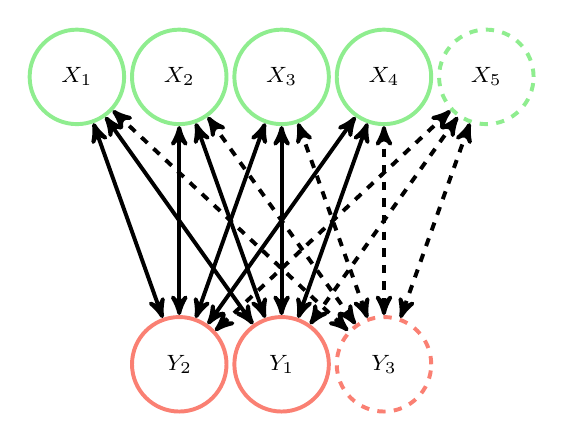
\begin{tikzpicture}[node distance=1.3cm, font=\footnotesize, align=center, >=stealth', line width=0.5mm]
        % Define colors
        \definecolor{lightgreen}{rgb}{0.56, 0.93, 0.56}
        \definecolor{lightred}{rgb}{0.98, 0.5, 0.45}

        % Nodes
        \node[draw, circle, draw=lightgreen, text=black, minimum size=1.2cm] (input1) {$X_1$};
        \node[draw, circle, draw=lightgreen, text=black, right of=input1, minimum size=1.2cm] (input2) {$X_2$};
        \node[draw, circle, draw=lightgreen, text=black, right of=input2, minimum size=1.2cm] (input3) {$X_3$};
        \node[draw, circle, draw=lightgreen, text=black, right of=input3, minimum size=1.2cm] (input4) {$X_4$};
        \node[draw, circle, dashed, draw=lightgreen, text=black, right of=input4, minimum size=1.2cm] (input5) {$X_5$};

        \node[draw, circle, draw=lightred, text=black, below=2.4cm of input3, minimum size=1.2cm] (output1) {$Y_1$};
        \node[draw, circle, draw=lightred, text=black, left of=output1, minimum size=1.2cm] (output2) {$Y_2$};
        \node[draw, circle, dashed, draw=lightred, text=black, right of=output1, minimum size=1.2cm] (output3) {$Y_3$};

        % Edges
        \foreach \i in {1,...,4} {
            \foreach \j in {1,...,2} {
                \draw[<->] (input\i) -- (output\j);
            }
        }
        \foreach \j in {1,...,2} {
            \draw[<->, dashed] (input5) -- (output\j);
        }
        \foreach \i in {1,...,5} {
            \draw[<->, dashed] (input\i) -- (output3);
        }
    \end{tikzpicture}
    \caption{\small Graphical representation of Bayesian Network where nodes $X_i$ represent the input variables and the nodes $Y_i$ represent the output variables to the analytical model. The solid lines represent the existing nodes in the model. Dashed line nodes representing those that are not present in the original model but can be added to the model as part of adapting the engineering environment as new information is gathered.}\label{fig:BN} 
    \vspace{-15pt}
\end{figure}


\subsection{Literature review}

Include your own work from previous paper and include work from Pavonne et al 2023. 

\section{Methodology}\label{sec:methodology}

Model is used as a tool to provide component decision support. 
\begin{enumerate}
    \item \textbf{Define objectives and constraints:} Here we define the objectives and constraints of the model.
    \item \textbf{Deterministic model:} This is the model that we are trying to replicate.
    \item \textbf{Select important parameters:} This is where parameters are selected for the surrogate model.
    \item \textbf{Data collection \& parameter estimation:} This is where the deterministic model is run to collect data that will be used to train the surrogate model.
    \item \textbf{Bayesian Network configuration:} This is where the Bayesian Network is configured to replicate the deterministic model.
    \item \textbf{Decision tree: exploration of new variables:} This is where we explore new variables that can be added to the model. 
    \item \textbf{Component decision support:} This is where the model is used to provide component decision support 
\end{enumerate}

\begin{figure*}[t]
    \centering
    \includegraphics[width=\textwidth]{figures/worflow_new.png}
    \caption{Workflow of the surrogate modelling process.}\label{fig:workflow}
\end{figure*}

\section{Results}\label{sec:Results} 

Addition of new data or information will be included. Addition of new node (child or parent) will be included. Addition of soft evidence will be included.

\section{Discussion}\label{sec:Discussion}


\section{Conclusion and Further Work}\label{sec:conc}


\section{Acknowledgments}
This research was supported by the EPSRC (Engineering and Physical Sciences Research Council, UK) Nuclear Energy Futures Centre for Doctoral. Training in Nuclear Energy (NEF CDT).  Other research studies under the NEF CDT involving Thomas Griffiths are supported in part by Tokamak Energy Ltd, UK. Views and opinions expressed are however those of the author(s) only a do not necessarily reflect those of Tokamak Energy Ltd.

\scriptsize\bibliographystyle{vancouver}
\scriptsize\bibliography{references.bib}

\end{document}